\section{Analyse du marché et des besoins, élaboration du cahier des charges}
Afin de developper un produit qui puisse convenir aux besoins des personnes souffrant de begaiement ainsi qu'aux othopédistes, j'ai effectué quelques recherches pour définir les exercices utilisés par les orthopédistes pour aider leurs patients. Le projet devant être developpé en seulement 12 semaines, j'ai décidé de concentrer mes recherches uniquement en ligne sans démarcher de réelles orthopédistes qui m'auraient permis de cerner plus précisement les besoins réelles mais qui m'aurait aussi pris beaucoup plus de temps.

J'ai également fait une étude comparative des applications actuellement disponible sur le marché des application Android, un tableau récapitulatif est disponible dans l'annexe \ref{appendix:market}. Cette étude a relevé un manque d'application complète qui propose plusieurs exercices, les applications se concentrent souvent sur un seul exercice. Aussi, aucune application propose de faire le lien entre les bègues et leurs thérapistes.

Afin de décrire complétement le but de l'application, le contexte d'utilisation dans lequel elle s'inscit (\textit{par qui ? comment ? pourquoi ?}), ses fonctionnalités et autres diverses exigences (sécurité, maintenabilité, etc),  j'ai rédigé un \textit{Software Requirements Specification (SRS)}. Un \textit{SRS} est un document décrivant les exigences fonctionelles et non fonctionnelles, les intéractions de l'utilisateurs sur le produit et les eventuelles contraintes à respecter (lois et regulations, protocole à utiliser, limitations matériel, etc.). La table des matière de ce document est disponible dans l'annexe \ref{appendix:srs}. En particulier, ce document décrit précisemment les interaction de l'utilisateur sur l'application récapitulées dans le diagramme de cas d'utilisation de la figure \ref{fig:srs}. L'annexe \ref{appendix:srs_example} contient un exemple de spécification d'un cas d'utilisation.

\begin{figure}
  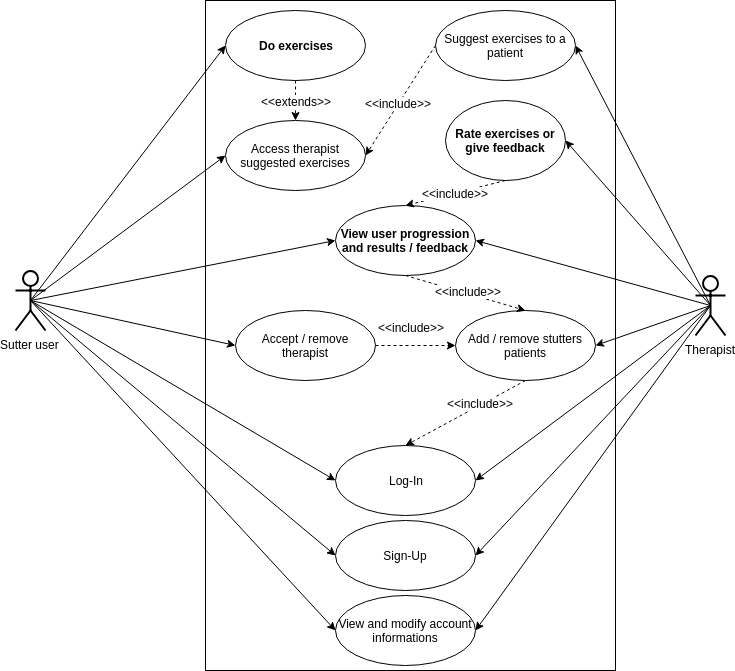
\includegraphics[width=.9\linewidth]{content/imgs/usecase.png}
  \caption{Diagramme cas d'utilisation}
  \label{fig:srs}
\end{figure}

\subsection{Résumé de cahier des charges de l'application}
\label{sec:resume_cdc}

L'application est destiné à être utilisé par des personnes souffrant de begaiement et par des orthopédistes.

Les bègues auront à disposition une liste d'exercices pour s'entrainer à mieux controler leur vitesse et leur rytme de parole. Chaque exercices sera paramétrable pour convenir aux besoins de l'utilisateur. En particulier les exercices pourront utiliser des resources que l'utilisateur devra lire, ces resources devront être récupérer via une collection de resources partagé possédant plusieurs type de resource : des mots, des phrases et des textes. Le bègue pourra choisir sur quelle type de resources il veut s'entrainer pour chaque exercices. Les exercices pourront d'appuyer aussi sur d'autres éléments tel qu'un enregistreur de voix, un enregistreur vidéo, etc. L'utilisateur pourra choisir d'activé ou non ces enregistreurs. Par exemple voici 4 exercices types qui rentre dans le cadre de l'application :

\begin{itemize}
  \item \textbf{Metronome} : laisser parler le bègue avec un metronome (un metronome est un appareil émettant un signal visuel et sonor à interval de temps régulier) ;
  \item \textbf{Reading} : laisser parler le bègue librement sur les resources de son choix (mots, textes, phrases) ;
  \item \textbf{Delayed Auditory Feedback (DAF)} : exercice où le bègue parle puis entend le retour de sa voix quelques dizaine de milliseconde après ;
  \item \textbf{Mirroring} : exercice où le bègue s'entraine à parler avec un retour vidéo de lui pour analyser ses mouvement facials.
\end{itemize}

L'utilisateur bègue pourra accéder à sa progression. La progression est consitué de l'historique de tous les exercices effectués. Ces exercices contiendront l'eventuel enregistrement de sa voix ou de sa caméra, les resources utilisé lors de cet exerice ainsi qu'un commentaire de son éventuel orthopédiste (voir ci-après). La progression de l'utilisateur pourra aussi être visualiser sous forme de courbe de pourcentage de réussite de prononciation des resources de l'exercice. L'utilisateur bègue pourra décidé de synchroniser des exercices dans le cloud. Pour ce faire il devra se créer un compte avec un nom, une adresse mail et un mot de passe. Une fois un exercice synchronisé dans le cloud, il sera accessible par son orthopédiste qui pourra alors ajouter un commentaire sur cet exercice. Ces utilisateurs peuvent donc ajouter un orthopédiste qui aura accès à tous leurs exercices synchronisés. Pour ajouter un orthopédiste ils devront connnaitre son identifiant personnel (voir ci-après). Ils pourront bien entendu révoquer l'accès de cet orhtopédiste aux exercices à tout moment.

Pour utiliser les fonctionnalités de l'application, les orthopédistes devront se créer un compte (comme pour les bègue, avec un nom, un courriel et un mot de passe). Une fois le compte créer ils auront accès à leur identifiants personnel ainsi que le liste de tous les utilisateurs bègue les ayant ajouté comme orthopédiste via leur application. Ces utilisateurs son appelé \textit{patients} pour l'orthopédiste. Un orthopédiste pourra visualisé la progression des ses patients. Il pourra aussi supprimer des patients de sa liste.















% eof
